\documentclass[Main.tex]{subfiles}
\begin{document}
\section{Probleemstelling}
Gebruikers hebben reeds de mogelijkheid om patroonherkenning te gebruiken op hun dataset. Toch kan de gebruiker op zoek zijn naar een wiskundige relatie tussen in zijn dataset in plaats van een patroon. De hypothese van dit onderzoek is de volgende "Er kan voor een gegeven dataset binnen beperkte tijd een passende vergelijking gevonden worden die voldoet aan de verwachtingen van de gebruiker.".

\subsection{Contextvrije grammatica}
Om wiskundige pattronen op te bouwen wordt er gebruikt gemaakt van een contextvrije grammatica. Volgens de \textit{formele taal theorie} \cite{cfg}
is een contextvrije grammatica een formele grammatica waarbij elke productieregel er uit ziet als volgt: $V \rightarrow w$. Hier staat $V$  voor \'e\'en niet-terminaal symbool is en $w$ een tekenreeks is van niet-terminale en terminale symbolen. Contextvrij betekend dat de productieregels kunnen toegepast worden los van de context waarin het niet-terminale symbool zich bevindt. \\

\begin{figure}[!htb]
\centering
\begin{framed}
$E \rightarrow E + E$ \\
$E \rightarrow E \ast E$ \\
$E \rightarrow a,b,\dotsc$
\end{framed}
\caption{Voorbeeld van contextvrije grammatica}
\label{fig:cfg}
\end{figure}

Als een andere wiskundige operatie gewenst is moet deze toegevoegd worden als een productieregel aan bovenstaande grammatica. Voordelig aan het werken met een context-vrije grammatica is de gemakkelijke aanpasbaarheid. Omdat de productieregels volledige onafhankelijk zijn van elkaar is het eenvoudig om de gewenste operaties door de gebruiker te laten defini\"eren. In de voorbeelden die hierna zullen volgen wordt de grammatica uit ~\ref{fig:cfg} gebruikt. De productieregels die gebruikt zullen worden in het algoritme bevatten $+, -, \ast, \div$ en \^{}.

\subsection{Boomstructuur}

Door herhaaldelijke toepassing van de productieregels onstaat er een boomstructuur. In deze boom bevinden zich alle mogelijke samenstellingen van productieregels die door de grammatica bepaald kunnen worden. Deze operatie zorgt voor een exponenti\"ele groei $r^{d}$ waarbij $d$ staat voor de diepte van de boom en $r$ voor het aantal productieregels van de vorm $E \rightarrow E$  $operand$ $ E$. De groei van deze boom staat uitgetekend in figuur \ref{fig:treeSize}.

\begin{figure}[!htb]
\centering
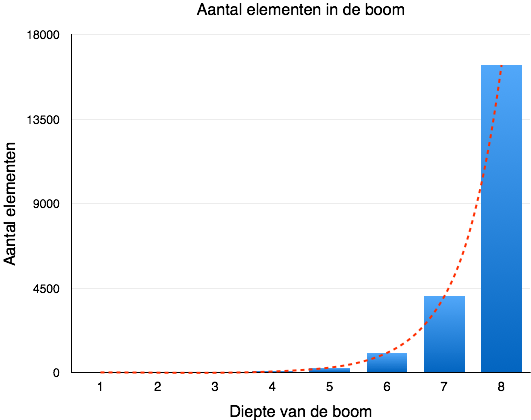
\includegraphics[width=\columnwidth]{treeSize.png}
\caption{Toename van het aantal knopen}
\label{fig:treeSize}
\end{figure}
Aangezien de groei van de boom exponentieel is bekomt men veel grotere berekeningstijden. Deze groei valt samen met de toename van de diepte in de boom. Het opstellen van de boom veroorzaakt een grote rekenkost. Dit heeft tot gevolg dat het ten zeerste aangeraden om deze boom slechts \'e\'enmalig op voorhand uit te werken.

\subsection{Evaluatiecriteria}

Snelheid, correctheid, gebruikersgemak en uitbreidbaarheid zijn de vier evaluatie criteria waarop het onderzoek gaat beoordeeld worden. Het doel van het onderzoek is dus een effici\"ent, correct en gemakkelijk uitbreidbaar algoritme te vinden dat uit een gegeven set van voorbeelden een geschikte vergelijking kan vinden. Ook het gebruikersgemak is van belang dat het het defini\"eren van wat de gebruiker juist van het algoritme verwacht eenvoudig is.
\end{document}